% !TeX root = ../thuthesis-example.tex

\chapter{研究现状与相关工作}

上一章总体介绍了大模型训练和微调过程中面临的效率挑战。
% 针对这个问题,本文从超参数、训练配方、扩展定律、性能预测定律、数据配置五个角度出发研究了可预测与训练技术,可以大幅提升大规模预训练的成功率和效率;从先验知识整合、参数高效微调、高效样本激活三个方面研究了低资源微调,可以大幅降低大语言模型在领域适配训练中的资源消耗和适配效率。
在本章中,我将介绍大模型的发展现状,研究背景和相关工作。


\section{Transformer架构}
自然语言处理领域的革命性突破始于2017年Transformer架构~\cite{Vaswani+2017}的诞生。这个由Vaswani等人提出的创新架构,彻底改变了传统序列建模的范式。其核心设计摒弃了循环神经网络(RNN)的时序依赖特性,转而采用全局注意力机制,这使得模型能够并行处理整个文本序列,训练效率提升达数十倍。当前最大规模的GPT-4~\cite{openai2023gpt4}、PaLM~\cite{chowdhery2023palm}等万亿参数模型,均建立在此基础架构之上。

% \begin{figure}
% \centering
% 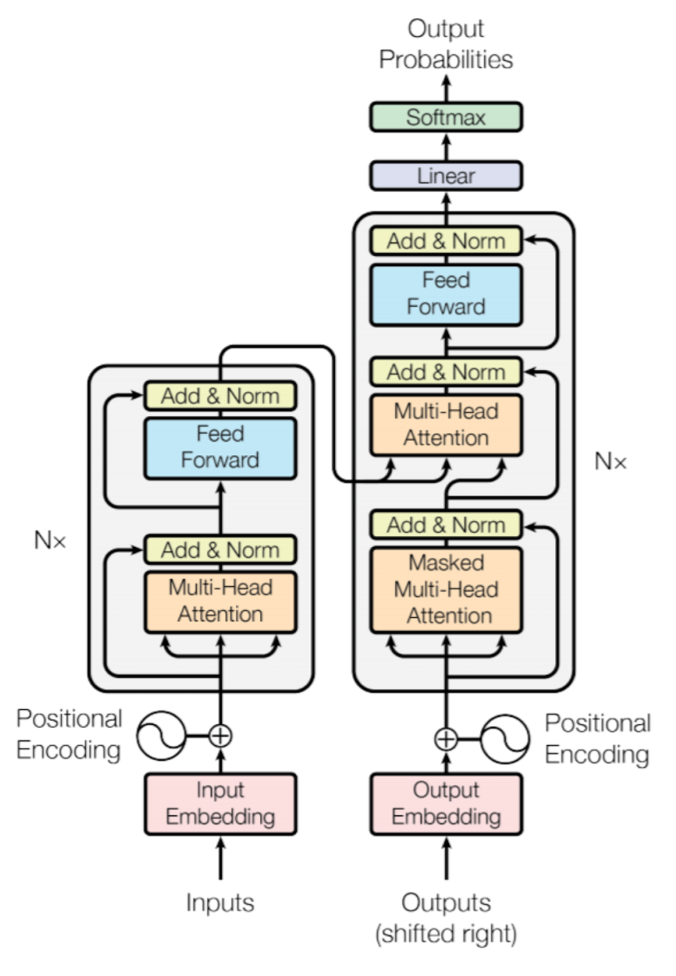
\includegraphics[width=0.5\linewidth]{misc/transformer.png}
% \caption{Transformer模型架构图}
% \label{fig:transformer}
% \end{figure}

每个Transformer层由两个关键模块协同工作:注意力机制与前馈网络。这种设计实现了对文本语义的多维度解析——注意力机制捕捉词语间的动态关联,前馈网络则负责特征的深度非线性转换。

\paragraph{注意力机制}
基础的注意力机制将输入$X$经过不同的线性变换变成三种张量$Q=XW_Q$,$K=XW_K$,$V=XW_V$,然后通过($Q$,$K$,$V$)三元组运算建立关联。其数学表达为:

\begin{equation}
    \text{Attention}(Q, K, V) = \text{Softmax}(\frac{QK^T}{\sqrt{d_h}})V
\end{equation}
其中$d_h$是$Q$、$K$、$V$ 表示的隐藏维度,归一化因子$\sqrt{d_h}$的引入有效缓解了高维空间中的梯度消失问题。

自注意力机制的精妙之处在于让输入序列自我参照。通过线性投影矩阵$W^Q$、$W^K$、$W^V$从输入表示$X$中生成差异化的特征空间,使得同一词语能同时承担查询者与被查询者的双重角色。这种设计使得模型可以建立跨越整个文本的语义关联,例如在“bank”的词义消歧中,模型能同时关注到河流或金融方面等上下文含义。

Transformer中还引入了多头注意力机制。将$d_{model}$维的嵌入空间分割为$h$个独立子空间(通常每个子空间的维度为64或者128),每个头学习不同的关联模式。这种设计类似于卷积神经网络中的多通道概念,允许模型并行捕获语法、语义、指代等不同类型的语言特征。其输出通过可学习的投影矩阵$W^O$实现特征融合,保证了维度的一致性。

\paragraph{前馈网络}
标准的双层前馈网络(FFN)通过激活函数实现特征变换:
\begin{equation}
    \text{FFN}(x) = \text{ReLU}(xW_1 + b_1)W_2 + b_2
\end{equation}
后来的研究者提出了门控前馈网络,在上述基础上引入门控机制:
\begin{equation}
    \text{GLU}(x) = (xW_1 \odot \sigma(xW_2))W_3
\end{equation}

其中$\sigma$代表激活函数,这种设计增强了模型对特征重要性的调节能力,在同等参数量下提升了模型性能。

本文建立于Transformer架构基础上,主要研究该架构下的高效预训练和微调方法。

\section{训练范式}
现代大语言模型的训练遵循“预训练+微调”的两阶段范式。这一范式随着BERT~\cite{devlin2018bert}、GPT~\cite{radford2018improving}、T5~\cite{raffel2020exploring}等模型的流行变成主流~\cite{xu2021pre}。预训练范式在历史上出现过多种,例如:
\begin{enumerate}
    \item 自回归预测(GPT系列):基于上文逐词预测,采用单向注意力掩码,适合文本生成任务;
    \item 掩码语言建模(BERT系列):随机遮蔽15\%的输入词元(token),利用双向上下文进行预测,擅长语义理解;
    \item 混合目标训练(T5、BART~\cite{lewis2019bart}):结合文本修复、句子重排等多种预训练任务,增强模型鲁棒性。
\end{enumerate}
现在比较主流的是第一种,即自回归预测,方式简单通用,接近自然语言交互模式。

在预训练过程中,模型在TB量级的词元化(tokenized)数据上进行大规模预训练,每一次大规模预训练都将花费巨量开销,因此训练次数的稀缺性成为了调整模型性能的瓶颈。而在预训练之后,模型会被微调,以适应下游任务。由于下游任务种类众多,并且通常在应用端进行,微调用户不具备大规模算力。本文在“预训练+微调”范式的两个阶段都做了相应的创新,以实现全流程的高效训练。

\section{损失扩展定律}
大量的深度学习训练都被观察到有所谓“扩展”现象\citep{hestness2017deep, kaplan2020scaling, rae2021scaling, aghajanyan2023scaling}。文献\citet{hestness2017deep}研究了基于循环神经网络(RNN)模型中损失的幂律扩展行为。\citet{kaplan2020scaling}描绘了基于Transformer的语言模型的损失扩展趋势,并探究了最优超参数的扩展行为。他们正式确立了如下扩展定律:
\begin{equation}
\label{eq:loss_scaling_law}
    L = c N^{-\alpha} + L_0
\end{equation}
其中\(N\)是模型(在他们的研究范围内特指语言模型)的非嵌入参数数量,\(c\)、\(\alpha\)为正系数,\(L_0\)是代表数据中随机性的不可约损失。这一公式推动了大语言模型的参数扩展。随后,针对各种领域和场景都建立了扩展定律,包括多模态\citep{henighan2020scaling, zhai2022scaling}、计算受限场景\citep{hoffmann2022training}、数据工程\citep{muennighoff2023scaling,sorscher2022beyond}以及强化学习\citep{gao2023scaling}等领域。\citet{yao2023research}通过引入超参数扩展方法,将该扩展定律扩展到跨超参数的损失预测领域。本文与现有文献存在两方面的联系。其一,这些文献主要聚焦于训练和验证时的损失指标,而这些指标并不能可靠地预测任务性能。本文基于这些扩展定律,扩展到任务性能的扩展定律。其二,本文第一次在大规模预训练场景下验证包含超参数扩展规律的全面扩展定律。


\section{任务性能的扩展行为}

尽管大语言模型的损失呈现可预测的下降趋势,但在模型扩展过程中,任务性能的提升却并非一帆风顺。虽然一些主要依赖知识记忆的任务呈现出逐步提升的态势,但随着模型规模的增大,众多任务展现出“涌现”能力\citep{srivastava2022beyond,wei2022emergent},即随着模型规模扩大,达到某一定阈值时,一些关键能力取得突飞猛进的进展。\citet{wei2022emergent}表明,“涌现”这一概念同样适用于诸如思维链\citep{wei2022chain}和上下文学习\citep{brown2020language}等提示学习技术,这使得理解任务性能的扩展定律变得更加复杂。似乎损失扩展定律并不能保证任务性能的提升,在预训练方法上也缺乏指导意义。
有几项研究致力于揭开这些涌现能力的神秘面纱。GPT-4的技术报告\citep{openai2023gpt4}称,GPT-4的任务性能可以用不到万分之一的计算量进行预测,不过并未披露具体方法,且承认某些能力仍然无法预测。另一项研究\citep{schaeffer2023emergent}将涌现归因于两个方面。第一个原因是非平滑指标导致的性能离散变化。本文对此并不认同,因为替代指标无法解释像精确匹配这样研究者最为关注的目标指标的突然提升。本文认同他们的第二个归因,即通过增加更多测试样本来提高分辨率。与他们的方法不同,本文提出了一种无需增加测试样本就能提高分辨率的实用方法。本文也是首次在开源环境下对任务性能的扩展行为进行定量研究的尝试,提出了任务扩展定律和加速涌现现象。 

\section{可扩展的预训练策略}

自从扩展定律\citep{hestness2017deep, kaplan2020scaling, rae2021scaling, aghajanyan2023scaling}被发现以来,人们从不同角度追求科学且可预测地\citep{achiam2023gpt,hu2023unlock, du2024understanding}扩大大语言模型的规模,尤其是在预训练阶段。预训练阶段容易有训练不稳定现象,为此,前人提出了张量程序(Tensor Program)系列工作\citep{yang2022tensor, yang2023tensor},以确保在不同模型规模下超参数的最优一致性。这种技术被用在训练CerebrasGPT\citep{dey2023cerebras}中。此外,\citet{wortsman2023small}建议利用较小的模型来预测并减轻较大模型训练中的不稳定性。从训练数据的角度来看,人们倡导了各种以数据为中心的策略\citep{xie2024doremi, shi2023context, ye2024data}。在训练方法领域,先前的研究深入探讨了各种学习率调度器(Learning Rate Scheduler)\citep{howard2018universal, raffel2020exploring, hundt2019sharpdarts},其中余弦退火学习率调度器(Cosine LRS)\citep{loshchilov2016sgdr}成为大语言模型中的主要选择。\citet{kaplan2020scaling,hoffmann2022training}精心研究了余弦退火学习率调度器的超参数,从而为后续的预训练工作奠定了基础。也有一些工作采用了非余弦退火学习率调度,例如DeepSeek\citep{bi2024deepseek}与本文提出的WSD学习率调度器有一定相似之处。关于批量大小调度,\citet{smith2017don}主张增加批量大小作为降低学习率的替代方法,这也是Yi-9B\citep{young2024yi}采用的策略。

\section{小规模语言模型}

本文使用多种可预测预训练技术,利用较少的资源预训练了一个小规模语言模型 (2.4B参数规模),其效果超过同期的Llama2-7B~\cite{touvron2023llama2},比肩Mistral-7B~\cite{jiang2023mistral}。
所谓“小语言模型”(SLMs),是一个不断演变的概念,随着时间推移经历了重大变革。目前,小语言模型通常被理解为与知名大语言模型相比规模较小的模型,其参数一般不超过70亿。这些模型的特点是能够在终端用户设备(如个人电脑和智能手机)上部署,即便没有图形处理器(GPU)也能运行。当前小语言模型领域的典型例子包括Phi系列\citep{gunasekar2023textbooks, li2023textbooks, Javaheripi2023Phi2}、TinyLlama\citep{zhang2024tinyllama}、MobileLLM\citep{liu2024mobilellm}以及Gemma\citep{Banks2024Gemma}等。 人们探索了多种方法来提高小语言模型的性能。这些方法包括使用高质量数据\citep{gunasekar2023textbooks, li2023textbooks, Javaheripi2023Phi2}、应用结构剪枝技术\citep{xia2023sheared},以及重新配置模型架构\citep{liu2024mobilellm}等。本文通过精心整合超参数优化、策略性训练方法、架构设计以及高质量数据,完成了小规模语言模型的高效训练。


\section{提示学习}
自从GPT-3~\cite{brown2020language}出现以来,提示学习(prompt-learning)受到了广泛关注。  
GPT-3表明,通过提示调优和上下文学习,大规模语言模型在低数据量情况下也能取得优异的性能。  
后续的研究~\cite{schick2020exploiting, schick2020s}指出,小规模语言模型~\cite{radford2018improving, devlin2019bert, liu2019roberta, lan2019albert}通过提示调优也能取得不错的表现。提示调优已被应用于多种任务,例如文本分类~\cite{schick2020exploiting}、自然语言理解~\cite{schick2020s, liu2021gpt}、关系抽取~\cite{han2021ptr,chen2021adaprompt}以及知识探测~\cite{petroni2019language, liu2021gpt}等。

标签词是提示调优中的重要组成部分,对提示调优的性能有显著影响~\cite{holtzman2021surface, gao2020making}。大多数研究使用人工编写的标签词~\cite{schick2020exploiting},这些标签词往往带有个人词汇的偏见且覆盖范围不足。其他一些研究~\cite{gao2020making, shin2020autoprompt,liu2021gpt,schick2020automatically}设计了自动标签词搜索方法以寻找更好的标签词选择,但这些方法需要充足的训练集和验证集进行优化。此外,自动确定的标签词通常是类别名称的同义词,这与本文通过外部知识库扩展标签词以涵盖多样化且全面的标签词的直觉有所不同。  
~\citet{schick2020automatically}和~\citet{shin2020autoprompt}也尝试为每个类别使用多个标签词。  
他们的标签词集合的最优大小通常少于10个,这在文本分类任务中缺乏足够的覆盖性。

\section{参数高效微调}
随着模型规模指数级增长,全参数微调面临严峻挑战。主要挑战有三点:1. 计算成本不菲,微调175B参数的GPT-3需要数百张GPU的算力 2. 储存成本高昂,储存微调后的大语言模型需要消耗和储存预训练模型一样大的空间开销。3. 过度微调会导致模型丧失通用能力,灾难性遗忘现象频发。在此背景下,参数高效微调(Parameter-efficient Tuning,又叫Delta Tuning~\cite{ding2022delta})应运而生。本文即与预训练模型的参数高效微调相关。参数高效微调只优化一小部分参数,而保留绝大多数参数不变,以低成本地适应下游任务。

早期的研究选择预训练模型进行部分微调~\cite{tajbakhsh2016convolutional, guo2020adafilter, guo2019spottune}。  
Adapter~\cite{houlsby2019parameter}是最早将参数高效微调方法应用于预训练语言模型的方法之一,它在每个Transformer层中插入线性神经模块,并取得了与全量微调相当的结果。  
随着近年来预训练语言模型规模的扩大,参数高效微调因其在计算和存储上的高效性而受到重视。这不仅催生了大量对Adapter的研究~\cite{pfeiffer2020adapterfusion,he2021effectiveness}
以及Adapter的变体~\cite{mahabadi2021compacter,sung2021vl},
还衍生出了一系列其他方法。  
Prefix tuning~\cite{li2021prefix}将嵌入向量附加到Transformer模型的隐藏状态前,而Prompt Tuning~\cite{lester2021power}进一步简化了这一策略,仅将此类嵌入向量附加到输入层。  
还有一些方法通过指定预训练模型中的部分参数为可训练参数来取得良好效果,例如Masking~\cite{zhao2020masking}、BitFit~\cite{zaken2021bitfit}、DiffPruning~\cite{guo2021parameter}等。另一流行的方法是LoRA~\cite{hu2021lora}。LoRA假设模型权重在微调后的变化本质上是低秩的,并使用可训练的秩分解矩阵进行模型微调。  
除了具体方法外,一些研究还对参数高效微调进行了探讨。~\citet{he2022unified}以统一的方式建模了多种方法,~\citet{ding2022delta}则提供了这些方法的理论讨论和全面的分析研究。  
本文提出在参数高效微调背景下的自动搜索可训练结构,这与上述所有工作的视角不同。在参数高效微调结构配置方面,AdapterDrop~\cite{ruckle-etal-2021-adapterdrop}基于手动试验探索了丢弃部分Adapter模块的方法。另一项工作~\cite{moosavi2022adaptable}通过在Adapter模块上学习开关来选择有益的Adapter模块,但该方法并未在预设的可训练参数数量下进行优化。此外,它们都局限于基于Adapter的方法。相比之下,本文提出的方法可以在受限的可训练参数预算下,在几乎所有参数高效微调模块的混合中进行搜索。  
%更多方法如DiffPruning、BitFit、prompt tuning等被开发


\section{神经架构搜索} 

本文在参数高效微调范围内进行结构搜索,这与神经架构搜索算法(Neural Architecture Search, NAS)相关。一类NAS算法使用强化学习或进化算法,通过从头训练结构并获取奖励来探索最佳结构~\cite{zoph2016neural, zoph2018learning,real2019regularized,pham2018efficient},这种方法通常消耗大量的计算资源。另一类NAS算法~\cite{liu2018darts, liang2019darts+, chen2019progressive}通过基于梯度的优化来解决这一问题。DARTS~\cite{liu2018darts}使用连续结构参数对离散结构进行松弛化,并通过梯度下降的方法进行优化。DARTS以更少的计算资源取得了具有竞争力的性能。本文从DARTS中汲取灵感,优化了结构参数。本文也是第一个在预训练骨干模型条件下进行NAS的研究。此外,本文还从带有二值门的NAS算法中汲取了灵感~\cite{cai2018proxylessnas, wu2019fbnet}。


